%%%%%%%%%%%%%%%%%%%%%%%%%%%%%%%%%%%%%%%%%%%%%%%%%%%%%%%%%%%%%%%%%%%%%%%%%%%%%%%%
%%%%%%%%%%%%%%%%%%%%%%%%%%%%%%%%%%%%%%%%%%%%%%%%%%%%%%%%%%%%%%%%%%%%%%%%%%%%%%%%

\section{Rap e musicalizar poesias}
\index{Musicalidade!Frase musical}

\begin{FraseFernandoPR}
A poesia é a linguagem, o que as equações são as matemáticas;
pois tentam explicar de uma forma curta e simples,
conceitos grandes e complexos. %(antes de 2013)
\end{FraseFernandoPR}

O objetivo nesta seção é aprimorar nossa habilidade na detecção da métrica numa peça musical,
especialmente a detecção do tempo forte da música.
Com esse proposito, procuraremos entender como um compositor musical utiliza a métrica,
em especial no momento que este deseja vincular música e letra;
é dizer, na \hyperref[sec:ProsodiaMusical]{\textbf{prosódia musical}}. 
Com esta tarefa em mente, aqui é proposto treinar usando duas estrategias:
\begin{itemize}
\item Musicalizar poesias; escolher um poema e agregar-lhe música.
\item Praticar rap no estilo livre; escolher uma música de acompanhamento e, em tempo real, 
 agregar-lhe letra num estilo recitativo.
\end{itemize}


\begin{tcbinformation} 
\textbf{RAP:}
\index{Música!RAP}
\label{ref:RAP}
 Este é um estilo de interpretação musical que apareceu na década de 1970;
o termo indicava originalmente o jeito estilizado de falar dos jovens afro-americanos, 
nas urbes dos Estados Unidos  \cite[pp. 1250]{latham2008diccionario}.
Atualmente, se entende que o rap é um estilo recitativo,
usado pelos ``rappers'' (pessoas que fazem rap),
onde surgem variações de tons na voz, 
provocadas pelas inflexões produzidas pela forma exagerada do uso da linguagem \cite[pp. 1250]{latham2008diccionario}.
\end{tcbinformation} 


\subsection{Musicalizar poesias}
\label{subsec:musicalizarpoesias}
Uma forma de treinar nossa percepção do acento métrico na música, 
é experimentar a perspetiva de um compositor que deseja musicalizar uma poesia.
Para mostrar este processo primeiro devemos escolher um poema ou verso,
como por exemplo o seguinte:

\begin{citando}
Vida simples, metáforas ao vento;\\
luzes cobertas, as lágrimas expostas.\\
Vida simples, lutas contra o tempo;\\
luta sorrindo, com lúdicas respostas.
\end{citando}

Uma vez escolhido o poema, 
devemos identificar as sílabas tônicas das palavras com significado;
é dizer as mais importantes, e associar essas sílabas a cada tempo forte num compasso;
como mostrado na Tabela \ref{tab:verso1}.

\begin{table}[h!]
\begin{center}
\begin{tabular}{|l||l||l||l|} % 
\hline
Compasso 1 & Compasso 2   & Compasso 3   & Compasso 4 \\ \hline \hline
\textbf{Vi}da       & \textbf{sim}ples, me- & \textbf{tá}foras ao    & \textbf{ven}to;  \\ \hline
\textbf{lu}zes  co- & \textbf{ber}tas, as   & \textbf{lá}grimas ex-  & \textbf{pos}tas. \\ \hline
\textbf{Vi}da       & \textbf{sim}ples, & \textbf{lu}tas contra o & \textbf{tem}po;  \\ \hline
\textbf{bri}lha, so-& \textbf{rrin}do, com   & \textbf{lú}dicas res-  & \textbf{pos}tas. \\ \hline
\end{tabular}
\caption{Separando o verso em compassos.}
\label{tab:verso1}
\end{center}
\end{table}

O seguinte passo é escolher uma frase rímica, que será repetida ciclicamente,
 e servirá como acompanhamento percussivo.
Esta frase nos ajudará a ter um sentido de localização para os tempos forte e fracos,
pelo que a principio quanto mais cíclico e simples seja esta, melhor;
porem não deve ser demasiado simples, 
pois uma frase demasiado repetitiva pode ser enjoativa ou desinteressante;
tendo estos dois polos, 
nós devemos fazer alguns compromissos e escolher, a nosso critério, um ponto intermediário. 
Assim, uma possível alternativa seria uma frase rítmica como a mostrada na Figura \ref{rap:emocional-protesto1},
que está composta por 4 compassos, como percebemos que era necessário, 
seguindo a Tabela \ref{tab:verso1}.

\begin{figure}[H]
\centering
    \centering
    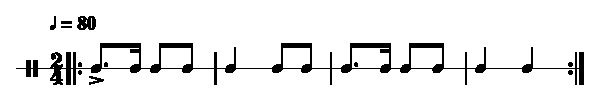
\includegraphics[width=0.99\textwidth]{chapters/cap-musicalidade-tecnica/rap-treino-1-1.eps}
\caption{Frase rítmica de 4 compassos, com final feminino.}
\label{rap:emocional-protesto1}
\end{figure}

Finalmente, tendo a base rítmica, podemos executar o texto de forma cantada,
ou recitativa como no caso do \hyperref[ref:RAP]{\textbf{rap}}.


\begin{comment}
Figura \ref{rap:emocional-protesto2}

\begin{figure}[H]
\centering
\begin{abc}[name=abc-emocional-protesto2]
X: 1 % start of header
K: C stafflines=1 % scale: C major
M: 2/4 %meter - compasso
Q:1/4=100
V:1 clef=perc stem=up %name="Pauta com clave de fá"   sname="Pauta com clave de fá"
[V:1] |:!>!B3/2 B/2 B1 B1| B3/2 B/2 B1 B1 | B2 B2| B2 z2:|
\end{abc}
\caption{Frase de 8 tempos, com palavra final aguda.}
\label{rap:emocional-protesto2}
\end{figure}
\end{comment}

\subsection{Praticar rap estilo livre}
\label{subsec:praticarrap}
A outra forma de treinar nossa métrica, 
é seguir o caminho oposto ao visto na Seção \ref{subsec:musicalizarpoesias}.
Neste caso, escolheremos primeiro uma base de rap\footnote{Podem ser achadas muitas ``bases de rap'',
livres e gratuitas na internet.}.
A Figura \ref{rap:base-rap} mostra um exemplo de uma base de rap.

\begin{figure}[H]
\centering
    \centering
    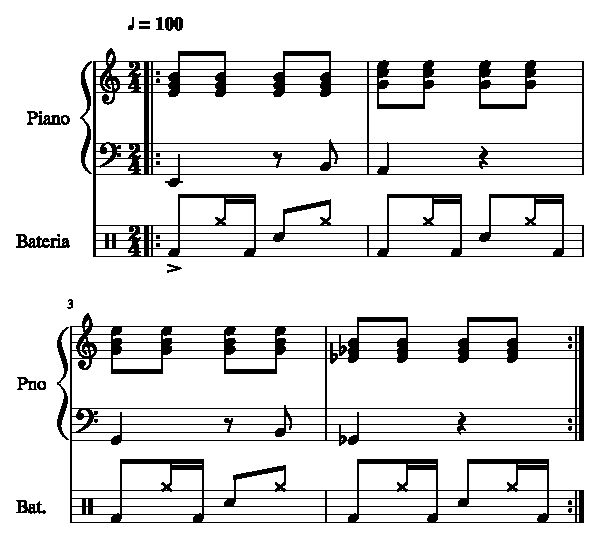
\includegraphics[width=0.99\textwidth]{chapters/cap-musicalidade-tecnica/base-rap-1.eps}
\caption{Base de rap.}
\label{rap:base-rap}
\end{figure}


Logo, de forma livre iremos falando expressando-nos  de forma recitativa;
é dizer ``rapeando'', tentando manter em todo momento um fio condutor no assunto tratado,
é procurando encaixar a sílaba tônica das palavras com conteúdo,
com o tempo forte da base de rap, seguindo as recomendações mostradas na Seção \ref{sec:ProsodiaMusical},
onde foi tratado o tema da \hyperref[sec:ProsodiaMusical]{\textbf{prosódia musical}}.
